\thispagestyle{empty}
\newgeometry{landscape, margin=1cm}
\footnotesize

\begin{landscape}
\begin{center}
\section*{Cheatsheet}
\end{center}
\begin{multicols*}{4}

\begin{tcolorboxTemplate}[title=Einfache Selektion: \texorpdfstring{\lstinline[style=sql]|SELECT|}{SELECT},colbacktitle=white, coltitle=black]
Auswahle einer oder mehrere Kolonnen:
\begin{lstlisting}[style=sql]
SELECT *
FROM users
\end{lstlisting}
\end{tcolorboxTemplate}

\begin{tcolorboxTemplate}[title=Duplikate entfernen: \texorpdfstring{\lstinline[style=sql]|SELECT DISTINCT|}{SELECT DISTINCT},colbacktitle=white, coltitle=black]
Auswahle einer oder mehrere Kolonnen:
\begin{lstlisting}[style=sql]
SELECT DISTINCT gender
FROM users
\end{lstlisting}
\end{tcolorboxTemplate}

\begin{tcolorboxTemplate}[title=Filter: \texorpdfstring{\lstinline[style=sql]|WHERE|}{WHERE},colbacktitle=white, coltitle=black]
Auswahle einer oder mehrere Kolonnen:
\begin{lstlisting}[style=sql]
SELECT name, city, gender
FROM users
WHERE gender="male"
\end{lstlisting}

\begin{table}[H]
\footnotesize
  \centering
  \begin{tabular}{c}
    \textbf{Operatoren} \\\midrule
    \texttt{=}                                    \\
    \texttt{<>}                                   \\
    \texttt{<}                                    \\
    \texttt{<=}                                   \\
    \texttt{>}                                    \\
    \texttt{>=}                                   \\
    \lstinline[style=sql]|BETWEEN x AND y|        \\
    \lstinline[style=sql]|IN (wert1, wert2, ...)| \\
    \lstinline[style=sql]|IS NULL|                \\
  \end{tabular}
\end{table}
\end{tcolorboxTemplate}

\begin{tcolorboxTemplate}[title=Ungefähre Treffer: \texorpdfstring{\lstinline[style=sql]|LIKE|}{LIKE},colbacktitle=white, coltitle=black]
Mit folgendem Befehl erhalten wir alle Städte, die mit ``Be...'' beginnen:

\begin{lstlisting}[style=sql]
SELECT DISTINCT city 
FROM users 
WHERE city LIKE "Be%"
\end{lstlisting}
\end{tcolorboxTemplate}

\begin{tcolorboxTemplate}[title=Sortieren: \texorpdfstring{\lstinline[style=sql]|ORDER BY|}{ORDER BY},colbacktitle=white, coltitle=black]
Mit folgendem Befehl erhalten wir alle Städte, die mit ``Be...'' beginnen:
\begin{lstlisting}[style=sql]
SELECT DISTINCT city 
FROM users 
ORDER BY city DESC
\end{lstlisting}
\begin{itemize}
\item \lstinline[style=sql]|DESC| = absteigend (\textit{descending})
\item \lstinline[style=sql]|ASC| = aufsteigend (\textit{ascending})
\end{itemize}
\end{tcolorboxTemplate}

\begin{tcolorboxTemplate}[title=Aggregatsfunktionen,colbacktitle=white, coltitle=black]
Mögliche Aggregatsfunktionen: \lstinline[style=sql]|COUNT, MAX, MIN, SUM, AVG LENGTH|
\end{tcolorboxTemplate}

\begin{tcolorboxTemplate}[title=Gruppieren: \texorpdfstring{\lstinline[style=sql]|GROUP BY|}{GROUP BY},colbacktitle=white, coltitle=black]
Anzahl Mitglieder pro Stadt:
\begin{lstlisting}[style=sql]
SELECT city, COUNT(*) AS "Mitglieder pro Stadt" 
FROM users 
GROUP BY city
\end{lstlisting}
\end{tcolorboxTemplate}

\begin{tcolorboxTemplate}[title=Filtern nach Gruppieren: \texorpdfstring{\lstinline[style=sql]|HAVING|}{HAVING},colbacktitle=white, coltitle=black]
Durchschnittliche Körpergrösse aller Mitglieder in jeder Stadt aus. Zeigen Sie nur die Städte, in denen die Menschen im Durchschnitt zwischen 150 und 155 gross sind.
\begin{lstlisting}[style=sql]
SELECT city, AVG(centimeters) AS "Durchschnittliche Körpergrösse"
FROM users
GROUP BY city
HAVING `Durchschnittliche Körpergrösse` BETWEEN 150 AND 155
\end{lstlisting}
\end{tcolorboxTemplate}

\begin{tcolorboxTemplate}[title=Erste / Letzte Zeilen: \texorpdfstring{\lstinline[style=sql]|LIMIT|}{LIMIT},colbacktitle=white, coltitle=black]
Drei Städte mit den meisten Mitgliedern:
    \begin{lstlisting}[style=sql]
SELECT city, COUNT(*) AS "Anzahl Mitglieder"
FROM users
GROUP BY city
ORDER BY `Anzahl Mitglieder` DESC
LIMIT 3
\end{lstlisting}
\end{tcolorboxTemplate}

\begin{tcolorboxTemplate}[title=Verzweigungen: \texorpdfstring{\lstinline[style=sql]|CASE WHEN|}{CASE WHEN},colbacktitle=white, coltitle=black]
Folgender Code berechnet für alle Männer, ob sie grösser, kleiner oder gleich dem Durchschnitt sind:

\begin{lstlisting}[style=sql]
SELECT name, centimeters,
CASE 
	WHEN centimeters > 179 THEN 'Gross'
    WHEN centimeters < 179 THEN 'Klein'
    ELSE 'Genau im Durchschnitt'
END AS Durchschnittlich
FROM users
WHERE gender="male"
\end{lstlisting}
\end{tcolorboxTemplate}

\begin{tcolorboxTemplate}[title=Mehrere Tabellen verbinden: \texorpdfstring{\lstinline[style=sql]|JOIN|}{JOIN},colbacktitle=white, coltitle=black]
\begin{figure}[H]
  \centering

  % INNER JOIN
  \begin{subfigure}[b]{0.23\textwidth}
    \centering
    \resizebox{\textwidth}{!}{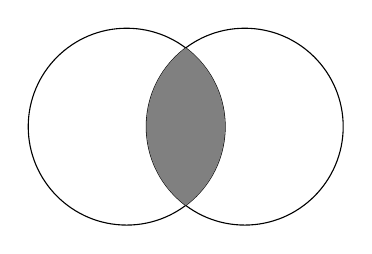
\begin{tikzpicture}
      \tikzset{circle node/.style={circle,draw=black, fill=none, minimum size=25mm, inner sep=0pt}}
      \node[circle node] (left) at (0,0) {};
      \node[circle node] (right) at (1.5,0) {};
      \begin{scope}
        \clip (0,0) circle (1.25cm);
        \fill[gray] (1.5,0) circle (1.25cm);
      \end{scope}
    \end{tikzpicture}}
    \caption{\lstinline[style=sql]|INNER|}
  \end{subfigure}
  % LEFT OUTER JOIN
  \begin{subfigure}[b]{0.23\textwidth}
    \centering
    \resizebox{\textwidth}{!}{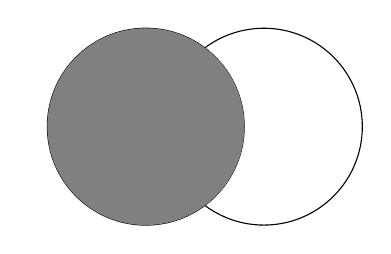
\begin{tikzpicture}
      \tikzset{circle node/.style={circle,draw=black, fill=none, minimum size=25mm, inner sep=0pt}}
      \node[circle node] (left) at (0,0) {};
      \node[circle node] (right) at (1.5,0) {};
      \begin{scope}
        \clip (-1.5,-1.25) rectangle (1.25,1.25);
        \fill[gray] (0,0) circle (1.25cm);
      \end{scope}
      \begin{scope}
        \clip (0,0) circle (1.25cm);
        \fill[gray] (1.5,0) circle (1.25cm);
      \end{scope}
    \end{tikzpicture}}
    \caption{\lstinline[style=sql]|LEFT|}
  \end{subfigure}
  % RIGHT OUTER JOIN
  \begin{subfigure}[b]{0.23\textwidth}
    \centering
    \resizebox{\textwidth}{!}{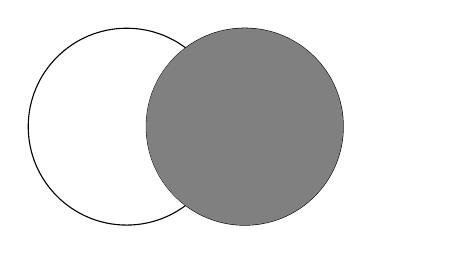
\begin{tikzpicture}
      \tikzset{circle node/.style={circle,draw=black, fill=none, minimum size=25mm, inner sep=0pt}}
      \node[circle node] (left) at (0,0) {};
      \node[circle node] (right) at (1.5,0) {};
      \begin{scope}
        \clip (0,-1.25) rectangle (4,1.25);
        \fill[gray] (1.5,0) circle (1.25cm);
      \end{scope}
      \begin{scope}
        \clip (1.5,0) circle (1.25cm);
        \fill[gray] (0,0) circle (1.25cm);
      \end{scope}
    \end{tikzpicture}}
    \caption{\lstinline[style=sql]|RIGHT|}
  \end{subfigure}
  % FULL OUTER JOIN
  \begin{subfigure}[b]{0.23\textwidth}
    \centering
    \resizebox{\textwidth}{!}{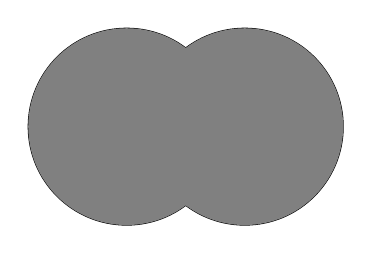
\begin{tikzpicture}
      \tikzset{circle node/.style={circle,draw=black, fill=none, minimum size=25mm, inner sep=0pt}}
      \node[circle node] (left) at (0,0) {};
      \node[circle node] (right) at (1.5,0) {};
      \fill[gray] (0,0) circle (1.25cm);
      \fill[gray] (1.5,0) circle (1.25cm);
    \end{tikzpicture}}
    \caption{\lstinline[style=sql]|FULL|}
  \end{subfigure}
\end{figure}
Syntax:
\begin{lstlisting}[style=sql]
SELECT kolonne1, kolonne2, ...
FROM tabelle1
INNER JOIN tabelle2
ON tabelle1.kolonne_id1 = tabelle2.kolonne_id2
\end{lstlisting}
\end{tcolorboxTemplate}

\begin{tcolorboxTemplate}[title=Tabellen erstellen: \texorpdfstring{\lstinline[style=sql]|CREATE table|}{CREATE table},colbacktitle=white, coltitle=black]
\begin{lstlisting}[style=sql]
CREATE TABLE tabellenname(
  kolonne1 eigenschaften1,
  kolonne2 eigenschaften2,
  ...
)
\end{lstlisting}
\end{tcolorboxTemplate}

\begin{tcolorboxTemplate}[title=Tabellen erstellen: \texorpdfstring{\lstinline[style=sql]|CREATE table|}{CREATE table},colbacktitle=white, coltitle=black]
\begin{lstlisting}[style=sql]
CREATE TABLE tabellenname(
  kolonne1 eigenschaften1,
  kolonne2 eigenschaften2,
  ...
)
\end{lstlisting}

\end{tcolorboxTemplate}

\begin{tcolorboxTemplate}[title=Daten einfügen: \texorpdfstring{\lstinline[style=sql]|INSERT|}{INSERT},colbacktitle=white, coltitle=black]
\begin{lstlisting}[style=sql]
INSERT INTO tabelle_name (kolonne1, kolonne2, kolonne3, ...)
VALUES (wert1, wert2, wert3, ...)
\end{lstlisting}
\end{tcolorboxTemplate}

\begin{tcolorboxTemplate}[title=Daten verändern: \texorpdfstring{\lstinline[style=sql]|UPDATE|}{UPDATE},colbacktitle=white, coltitle=black]
\begin{lstlisting}[style=sql]
UPDATE tabelle_name
SET kolonne1 = wert1, kolonne2=wert2, ...
WHERE bedingung(en)
\end{lstlisting}
\end{tcolorboxTemplate}

\begin{tcolorboxTemplate}[title=Einträge löschen: \texorpdfstring{\lstinline[style=sql]|DELETE FROM|}{DELETE FROM},colbacktitle=white, coltitle=black]
\begin{lstlisting}[style=sql]
DELETE FROM users
WHERE username="guenther37"
\end{lstlisting}
\end{tcolorboxTemplate}

\end{multicols*}
\end{landscape}
